\documentclass{svproc}
% \usepackage[utf8]{inputenc

% Required packages by SVProc class
\usepackage{multicol}
\usepackage{footmisc}

% Various packages
\usepackage{float}
\usepackage{comment}
\usepackage{array}
\usepackage{graphicx}
\usepackage{booktabs}
\usepackage{graphicx}
\usepackage{cite}

% Various math packages
\usepackage{amsmath}								
\usepackage{amssymb}
\usepackage{latexsym}
\usepackage{amsthm}
\usepackage{bm}
\usepackage{commath}
\usepackage{float}
\usepackage{units}
\usepackage{mathtools}

% packages for drawings
\usepackage{tikz}
\usetikzlibrary{arrows,shapes,trees,calc}
\usetikzlibrary{backgrounds}
\usepackage{pgfplots}
\pgfplotsset{compat=1.15}
\usepgfplotslibrary{polar}
\usepgfplotslibrary{patchplots}

%% downsample images to make file smaller
%\usepackage{epstopdf}
%\epstopdfDeclareGraphicsRule{.pdf}{png}{.png}{convert #1 \OutputFile}
%\DeclareGraphicsExtensions{.png,.pdf}

% packages for 3d plotting with tikz
\usepackage{tikz-3dplot} %requires 3dplot.sty to be in same directory, or in your LaTeX installation
%\usepackage[active,tightpage]{preview}  %generates a tightly fitting border around the work
%\PreviewEnvironment{tikzpicture}
%\setlength\PreviewBorder{2mm}

% % Commands for theorems (already defined in SVProc class)
% \newtheorem{definition}{Definition}[section]
% \newtheorem{theorem}{Theorem}[section]
% \newtheorem{assumption}{Assumption}[section]

% Definitions of custom colors
\definecolor{lightyellow}{RGB}{255,236,132}
\definecolor{lightgreen}{RGB}{161,239,10}
\definecolor{darkgreen}{RGB}{61,124,68}
\definecolor{lightblue}{RGB}{72,131,219}
\definecolor{darkblue}{RGB}{39,63,186}
\definecolor{plgreen}{RGB}{27,158,119}
\definecolor{plorange}{RGB}{217,95,2}
\definecolor{plpurple}{RGB}{117,112,179}
\definecolor{plpink}{RGB}{231,41,138}

% Editing tools
\usepackage{color}  % For Highlighting
\newcommand{\hilight}[1]{\colorbox{yellow}{#1}}
\newcommand{\David}[1]{\textcolor{red}{(#1)}}
\newcommand{\Ram}[1]{\textcolor{blue}{(#1)}}
\newcommand{\Dan}[1]{\textcolor{magenta}{(#1)}}
\newcommand{\Audrey}[1]{\textcolor{maroon}{(#1)}}

% Set macros to make certain things easier
\newcommand{\mtx}[1]{\begin{bmatrix} #1 \end{bmatrix}}
\newcommand{\J}{\bar{J}}
\newcommand{\C}{\bar{C}}
\newcommand{\x}{\vec{x}}
\newcommand{\q}{\vec{q}}
\newcommand{\p}{\vec{p}}
\newcommand{\T}{\vec{\tau}}
\newcommand{\f}{\vec{f}}
\newcommand{\V}{\vec{V}}
\newcommand{\tx}[1]{\text{#1}}
\newcommand{\D}{\bar{\mathcal{D}}}

\graphicspath{figures/}
\DeclareGraphicsExtensions{.pdf,.jpeg,.png}

\begin{document}
\mainmatter
\title{Model-Based Position Control of Parallel Combinations of Fluid-Driven Soft Actuators}
\titlerunning{Control of Parallel Combinations of Soft Actuators}
\author{Daniel Bruder \and C. David Remy \and Ram Vasudevan}
\tocauthor{Daniel Bruder, C. David Remy, and Ram Vasudevan}
\authorrunning{Daniel Bruder et al.}
\institute{University of Michigan, Ann Arbor MI 48109, USA,\\
\email{bruderd@umich.edu}}
\maketitle

% \begin{abstract}
    (Abstract goes here)
\end{abstract}
% \newpage
\section{Motivation}    \label{sec:motivation}
% Motivation, problem statement, related work

%% Problem statement
% Soft robotic systems require methods of actuation that do not inhibit their compliant structure. Parallel combinations of fiber-reinforced fluid-driven actuators are capable of generating controllable spacial forces without imposing rigidity.

%% What are soft robots, why are they useful?
Soft robotic systems have the potential to offer capabilities that go far beyond those of traditional rigid-bodied robots.
Their compliant structure allows them to adapt their overall shape to navigate unstructured environments, to safely work alongside humans, to manipulate delicate goods, and to absorb impacts without damage \cite{majidi2014soft}. 

%% Fluid-driven actuators are a good choice for soft robots
To obtain all of these advantages, soft robotic systems require actuators that can produce forces without imposing a rigid structure. As a result, a large number of soft robotic systems are actuated by fluid-driven soft actuators \cite{grissom2006design, hawkes2017soft, marchese2014autonomous, tolley2014resilient}. 
In these actuators, a pressurized fluid such as water or air induces a targeted deformation of a soft structure enclosing a fluid-filled cavity. 
To achieve a specific type and direction of deformation, and not merely a homogeneous expansion, the stiffness of the soft structure is pattered by adding reinforcing elements such as fibers, beams, or plates \cite{galloway2013mechanically, marchese2015recipe, rus2015design}.

%% Existing literature on the control of soft robots rely mainly on feed-forward control (with some notable exceptions). Goal of this paper is to demonstrate the capability of a model-based approach to achieve control
The most common approach to controlling systems that are actuated by fluid-driven soft actuators is model-free feed-forward, such as in soft crawling robots (cite), fish (cite), etc (include more examples and citations). Such an approach is sufficient to demonstrate the novel capabilities of a soft structure or to generate repeated motions, but falls short in more complex tasks where non-periodic position/force control is desired. \Dan{Should probably also mention model-free PID} 

%% Model-based control approach enables control of more complex behavior
In this work we propose and validate a model-based control approach founded on the notion of a \emph{fluid Jacobian}, which linearly maps the geometrical deformation of a soft actuator, or of a system of actuators, to a change in their volume. 
Due to its linear structure, this model enables the efficient numerical calculation of control inputs given a desired state.
%The linear structure of this model enables efficient calculation of control inputs given a desired state.
%% FREEs are customizable and well-suited for parallel combinations
We demonstrate the efficacy of this approach by controlling the position of an end effector connected to a parallel configuration of cylindrical fiber-reinforced soft actuators, known as Fiber-Reinforced Elastomeric Enclosures (FREEs), which are capable of exerting forces along their central axis and moments about it, based on the angle at which their fiber reinforcements are wound \cite{bishop2015design, connolly2015mechanical, felt2018closed, krishnan2015kinematics, bishop2013force, bruder2017model, sedal2017constitutive}.






% FREEs are used due to their versatility, % customizability?  
% since by merely changing the arrangement of a FREE's fiber reinforcements, it can be customized to yield a desired motion or force profile without constraining motion to occur exclusively in the direction of force \cite{bishop2015design, connolly2015mechanical, felt2018closed, krishnan2015kinematics, bishop2013force, bruder2017model, sedal2017constitutive}. This property makes them well suited to be combined in parallel, where the forces of individual actuators are superimposed to generate a multidimensional spacial force (cite IROS). 
% \Dan{I want it to be clear that the approach we use is not specific to FREEs, we have just chosen them to demonstrate our model. But I don't know if introducing them at the end of the section like this is best.}


%% TEXT FROM IROS PAPER FOR REFERENCE %%%%%%%%%%%%%%%%%%%%%%%%%%%%%%%%%%%%%%%%%%%%%%%%%%%%%%%%%%%%%

% Examples of these actuators include bellows \cite{pridham1967bellows}, pneu-nets \cite{mosadegh2014pneumatic}, McKibben muscles \cite{tondu2012modelling}.

%% FREEs are great because they are fluid-driven and customizable
%A particularly promising type of soft fluid-driven actuator is the fiber-reinforced elasomeric enclosure (FREE) \cite{bishop2015design}. 
%A FREE consists of a fluid-filled elastomeric tube wound with reinforcing fibers that pattern its stiffness to yield a desired mode and direction of deformation upon pressurization. %(Fig.~\ref{fig:FREEhand}). 
%By changing the arrangement of these fibers, a FREE can be customized to yield a variety of desired deformations and forces \cite{bishop2015design}. 


%% Basic argument: Rigid robots: structure constrained, actuators exert forces at joints to move structure,  Soft robots: structure unconstrained, actuators impose forces/constraints to move structure
%Due to their soft and deformable structure, FREEs (and fluid driven soft actuators in general) differ in a fundamental way from traditional actuators.
%An electric motor, for example, essentially combines a kinematic constraint (the rotation axis of the motor, which is physically defined by a pair of bearings) with a force generating element (the electromagnetic forces, which create the motor torque).
%Since the motion of such an actuator is inherently limited to one dimension, multiple actuator stages are typically combined in \emph{series} to achieve multi degree of freedom (DOF) motions. 
%This is the prevalent design, for example, in industrial robotic arms.
%In contrast, in a soft actuator, the force generating element is not supported by any physical kinematic constraints.
%The actuator produces a spatial force without constraining the motion to happen exclusively in the direction of this force.
%Because of this, soft actuators are particularly well suited to be combined in \emph{parallel}, where the forces of the individual actuators are superimposed to generate a multi-dimensional spatial force.
%Such parallel combinations enable particularly compact designs of multi-DOF motion stages.
%They have equivalents in the world of traditional robotic systems, such as the well-known Steward Platform.
%However, in such systems, the complexity is much higher, as each individual actuator needs to be combined with five additional joints to overcome the inherent kinematic constraints.


%% Outline of paper
%This paper explores the potential of combining different types of FREE actuators in parallel to achieve fully controllable spatial forces.
%This work thus expands on the existing literature regarding fiber-reinforced fluid-driven actuators, which has focused mainly on the kinematics  \cite{bishop2015design, connolly2015mechanical, felt2018closed, krishnan2015kinematics} or kinetics \cite{bishop2013force, bruder2017model, sedal2017constitutive} of individual actuators, or the kinematics of parallel combinations of actuators \cite{bishop2012parallel, bishop2012parallelsynth}.
%Here, we study which combinations and configurations of FREEs enable effective control of multi-DOF forces.
%To this end, we present a novel way to represent and calculate actuator forces in terms of a state dependent fluid-Jacobian.
%This concept readily extends from a single soft actuator to parallel combinations of actuators.
%Our design and modelling methodology is employed and evaluated experimentally on a two degree of freedom test bench.



% %% Existing literature 
% Existing literature regarding fiber-reinforced fluid-driven actuators has focused on modeling the kinematics  \cite{bishop2015design, connolly2015mechanical, felt2018closed, krishnan2015kinematics} and kinetics \cite{bishop2013force, bruder2017model, sedal2017constitutive} of individual actuators, or the kinematics \cite{bishop2012parallel, bishop2012parallelsynth} and kinetics cite(BRUDER IROS) of parallel combinations of actuators . The aim of this work is to extend this work to control robotic systems that are actuated by parallel combinations of FREEs.




\newpage
\section{Technical Approach}    \label{sec:technical-approach}
% Technical Approach

%% We control end effector by controlling actuator pressures
A parallel combination consists of several actuators arranged such that one end is attached to a common ground while the other is attached to a common end effector. We desire to control the position of that end effector by varying the internal pressures inside of the actuators. For a desired end effector position, we use a force balance model to solve for a corresponding set of actuator pressures.

%% End effector forces can be written as a function of pressure and state
With the internal pressure and displacements of the actuators described by state vectors $\p$ and $\q$, respectively, the position and orientation of the end effector described by a state vector $\x$, and assuming that an inverse kinematics function $\q(\x)$ allows the computation of  $\q$ in terms of $\x$ , the end effector force $\f$ can be expressed in terms of $\x$ and $\p$ as 
\begin{align}
    \f (\x, \p) &= \J_x^T (\x) \p + \f_{\tx{elast}} \left( \q(\x) \right),
\end{align}
where $\J_x = \frac{\partial \vec{V}}{\partial \x}$ is the \emph{fluid Jacobian} which relates the change in volume of the actuators $\V$ to the change in the state of the end effector $\x$ (cite: IROS).

%% Solving for equilibrium points
This expression enables us to determine the pressure required to actuate the system toward a desired equilibrium state, $\x_\tx{des}$, by solving the following equation for $\p$,
\begin{align}
    0 &= \f (\x_{\tx{des}}, \p) + \f_\tx{load} =  \J_x^T (\x_\tx{des}) \p + \f_{\tx{elast}} \left( \q(\x_\tx{des}) \right) + \f_\tx{load} , 
    \label{eq:pequation}
\end{align}
where $\f_\tx{load}$ is the force imposed by external loads.
Since \eqref{eq:pequation} is a linear equation in $\p$, it is amenable to efficient numerical solving methods. In principle, \eqref{eq:pequation} may have multiple solutions, so we restructure it as a quadratic program that minimizes the magnitude of the pressure input with inequality constraints ensure that the minimizer solves \eqref{eq:pequation} to within a desired tolerance, tol.

\begin{equation}
\begin{aligned}
    & \underset{\p}{\text{minimize}}
    & & \p^T Q \p \\
    & \text{subject to}
    & & \mtx{\J_x^T \\ 
            -\J_x^T \\
            -\text{I} \\ \text{I}} \p
        \leq 
        \mtx{- \left( \f_{\tx{elast}} + \f_\tx{load} \right) + \text{tol} \\
            \f_{\tx{elast}} + \f_\tx{load} + \text{tol} \\
            -\p^\text{min} \\ \p^\text{max}}
\end{aligned}
\end{equation}

This quadratic program can be performed quickly enough to enable equilibrium position control of the end effector by iterative solving \eqref{eq:pequation} in real time.
















































%% TEXT FROM IROS PAPER FOR REFERENCE %%%%%%%%%%%%%%%%%%%%%%%%%%%%%%%%%%%%%%%%%%%%%%%%%%%%%%%%%%%%%

%\subsection{Model of a Parallel Combination of FREEs}
%The net force generated by parallel combinations of FREEs at the end effector (mostly following conventions of the IROS paper)
%\begin{align}
%    \f(\q, \p) &= \sum_{i=1}^n \f_{i} = \sum_{i=1}^n \D_i \T_i \\
%    &= \sum_{i=1}^n \D_i \left( \J^T_{q, i} (\q_i) p_i + \C_{q, i} \q_i \right) \\
%    &= \sum_{i=1}^n \bar{J}^T_{x, i} (\vec{x}) p_i + \C_{x, i} \q_i(\x),
%\end{align}
%where $\J_{x, i} = \J_{q, i} \D_i^T$ is the fluid Jacobian of the $i$th FREE expressed in end effector coordinates and $\C_x = \D_i \C_{q, i}$ is the stiffness contribution of the the $i$th FREE on the stiffness of the end effector. 
%This can be written compactly in matrix notation as
%\begin{align}
%    \f (\x, \p) &= \J_x^T (\x) \p + \C_x \q(\x)
%\end{align}
%with the overall fluid Jacobian $\J_x$ and overall stiffness $\C_x$
%\begin{align}
%    \J_x &= \mtx{\J^T_{x, 1} & \J^T_{x, 2} & \cdots & \J^T_{x, n}}^T \\
%    \C_x &= \mtx{\C_{x,1} & \C_{x,2} & \cdots & \C_{x,n}}
%\end{align}

\newpage
\section{Results}   \label{sec:results}
% Results

%% Able to approximate the feasable control region by solving QP over large displacement space

%% Can do steady state control of 2dof system to within ____ m displacement and ____ degrees rotation

%% Plot comparing the the desired end effector positions to those achieved
\begin{figure}
    \centering
    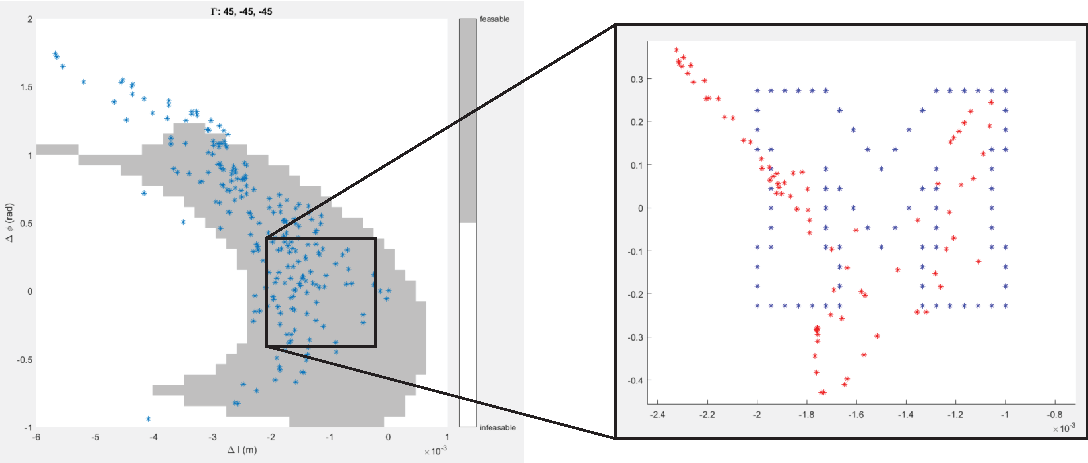
\includegraphics[width=\linewidth]{figures/resultsDiagram.pdf}
    \caption{(a) The feasable control region calculated by the model with measured test points over range of admissable pressures superimposed. (b) Desired end effector positions compared to measured end effector positions at corresponding pressures. \Dan{Placeholder figure and caption just to show the proposed structure. Didn't want to waste time nicely formatting bad results.}}
    \label{fig:results}
\end{figure}


\newpage
\section{Experiments}   \label{sec:experiments}
% Experiments

We evaluate the model-based position control approach proposed in section \ref{sec:technical-approach} by applying it to a real system composed of FREE actuators in parallel, and measuring the error in tracking a set of desired end effector states. 

%In order to evaluate the model-based position control approach proposed in section \ref{sec:technical-approach}, we use our model to compute the pressure inputs needed to achieve a set of end effector positions, then measure the error 

%% Description of system identification
Our model requires experimental system identification of the elastomer force, $\f_\tx{elast}$, from \eqref{eq:pequation}. This is done by measuring the end effector position $\x'$ over a random sampling of control pressures $\p'$, calculating $\f_\tx{elast}' = - \left( \J_{\x}^T (\x') \p' + \f_\tx{load} \right)$ at each point, then approximating $\f_\tx{elast} (\x)$ as 2nd degree polynomial of $\x$ using least-squares regression.

%% Summary of experimental procedure
We approximate the workspace of the system via the process explained in section \ref{sec:technical-approach}. We then define a set of desired end effector states within the computed workspace and solve \eqref{eq:QP} to find suitable pressure inputs to achieve each one. We measure the actual state of the system under these input pressures, and compare the measured states to the desired ones. We quantitatively characterize the performance of our model-based control strategy with both the root-mean-square error and maximum error over all points tested. Preliminary results of this kind are presented in section \ref{sec:results}.


%% figure: the 2dof and 3dof modules, labeled, side to side
\begin{figure}
    \centering
    \begin{tikzpicture}
        \def\colWidth{0.4\linewidth}
        \matrix [row sep=0.5cm, column sep=1cm, style={align=center}] (my matrix) at (0,0)
        {
        \node[style={anchor=center}] {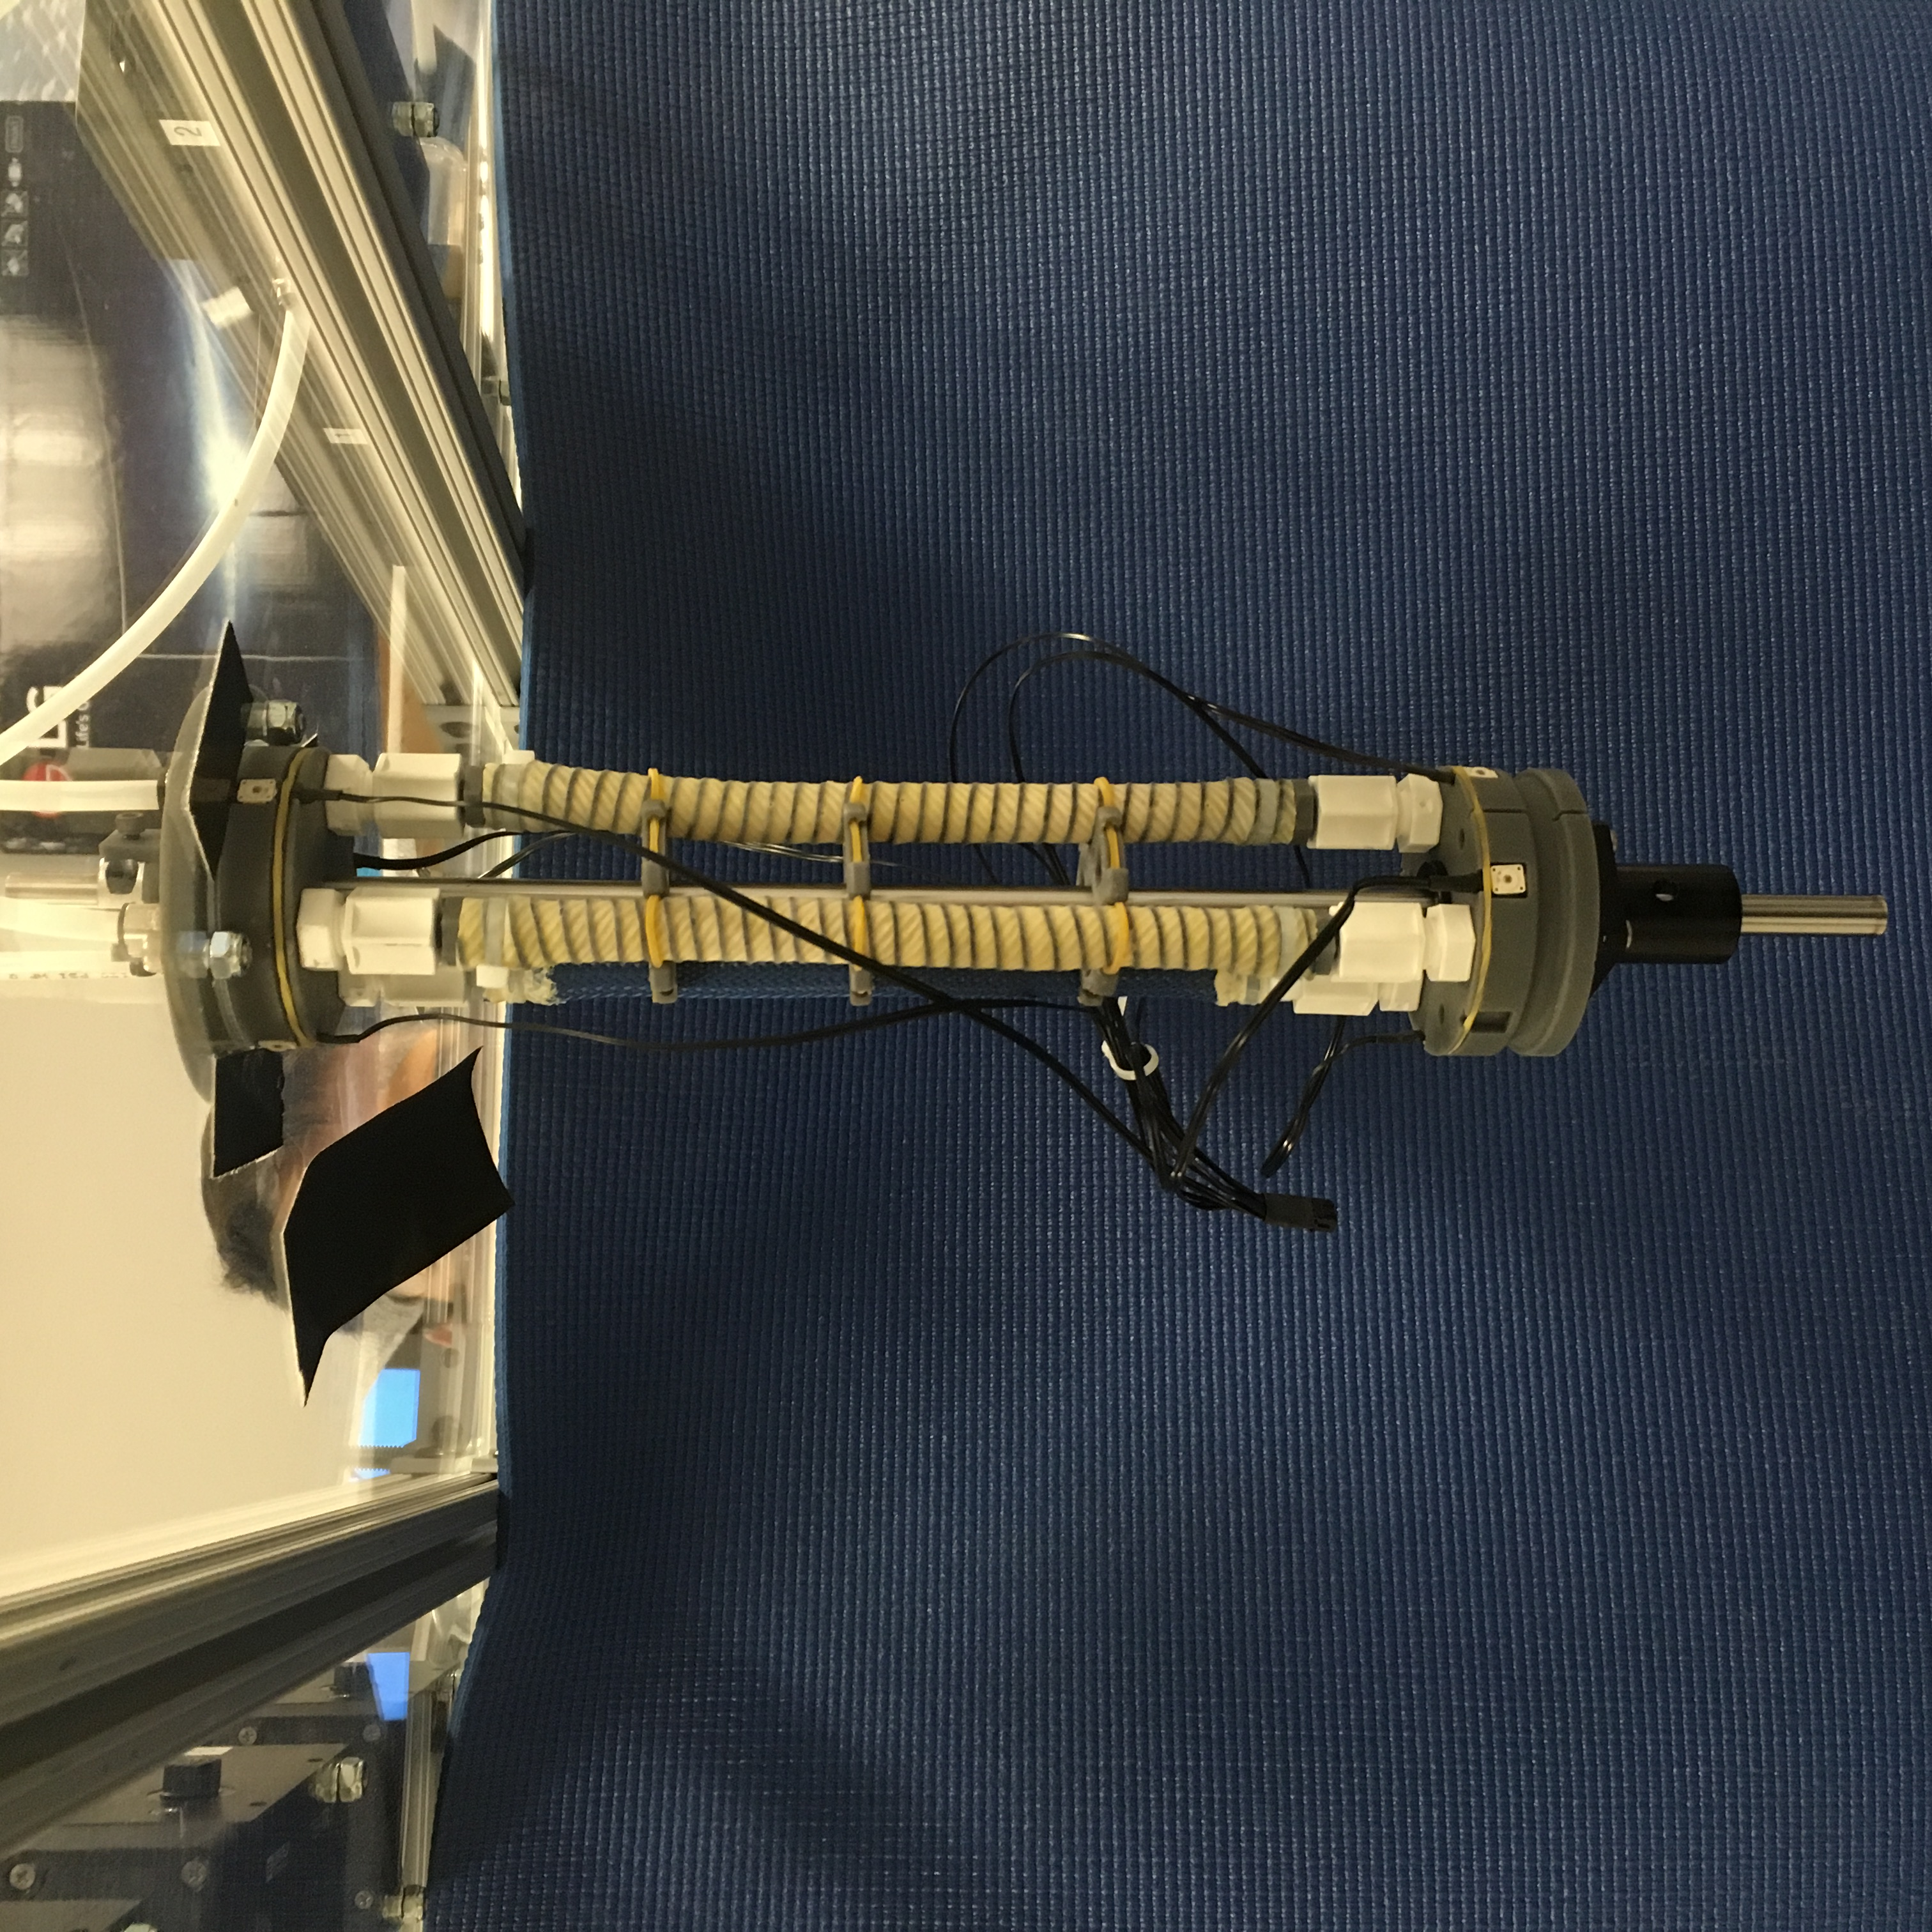
\includegraphics[width=\colWidth, angle=-90]{figures/free3.JPG}};
        &
        \node[style={anchor=center}] {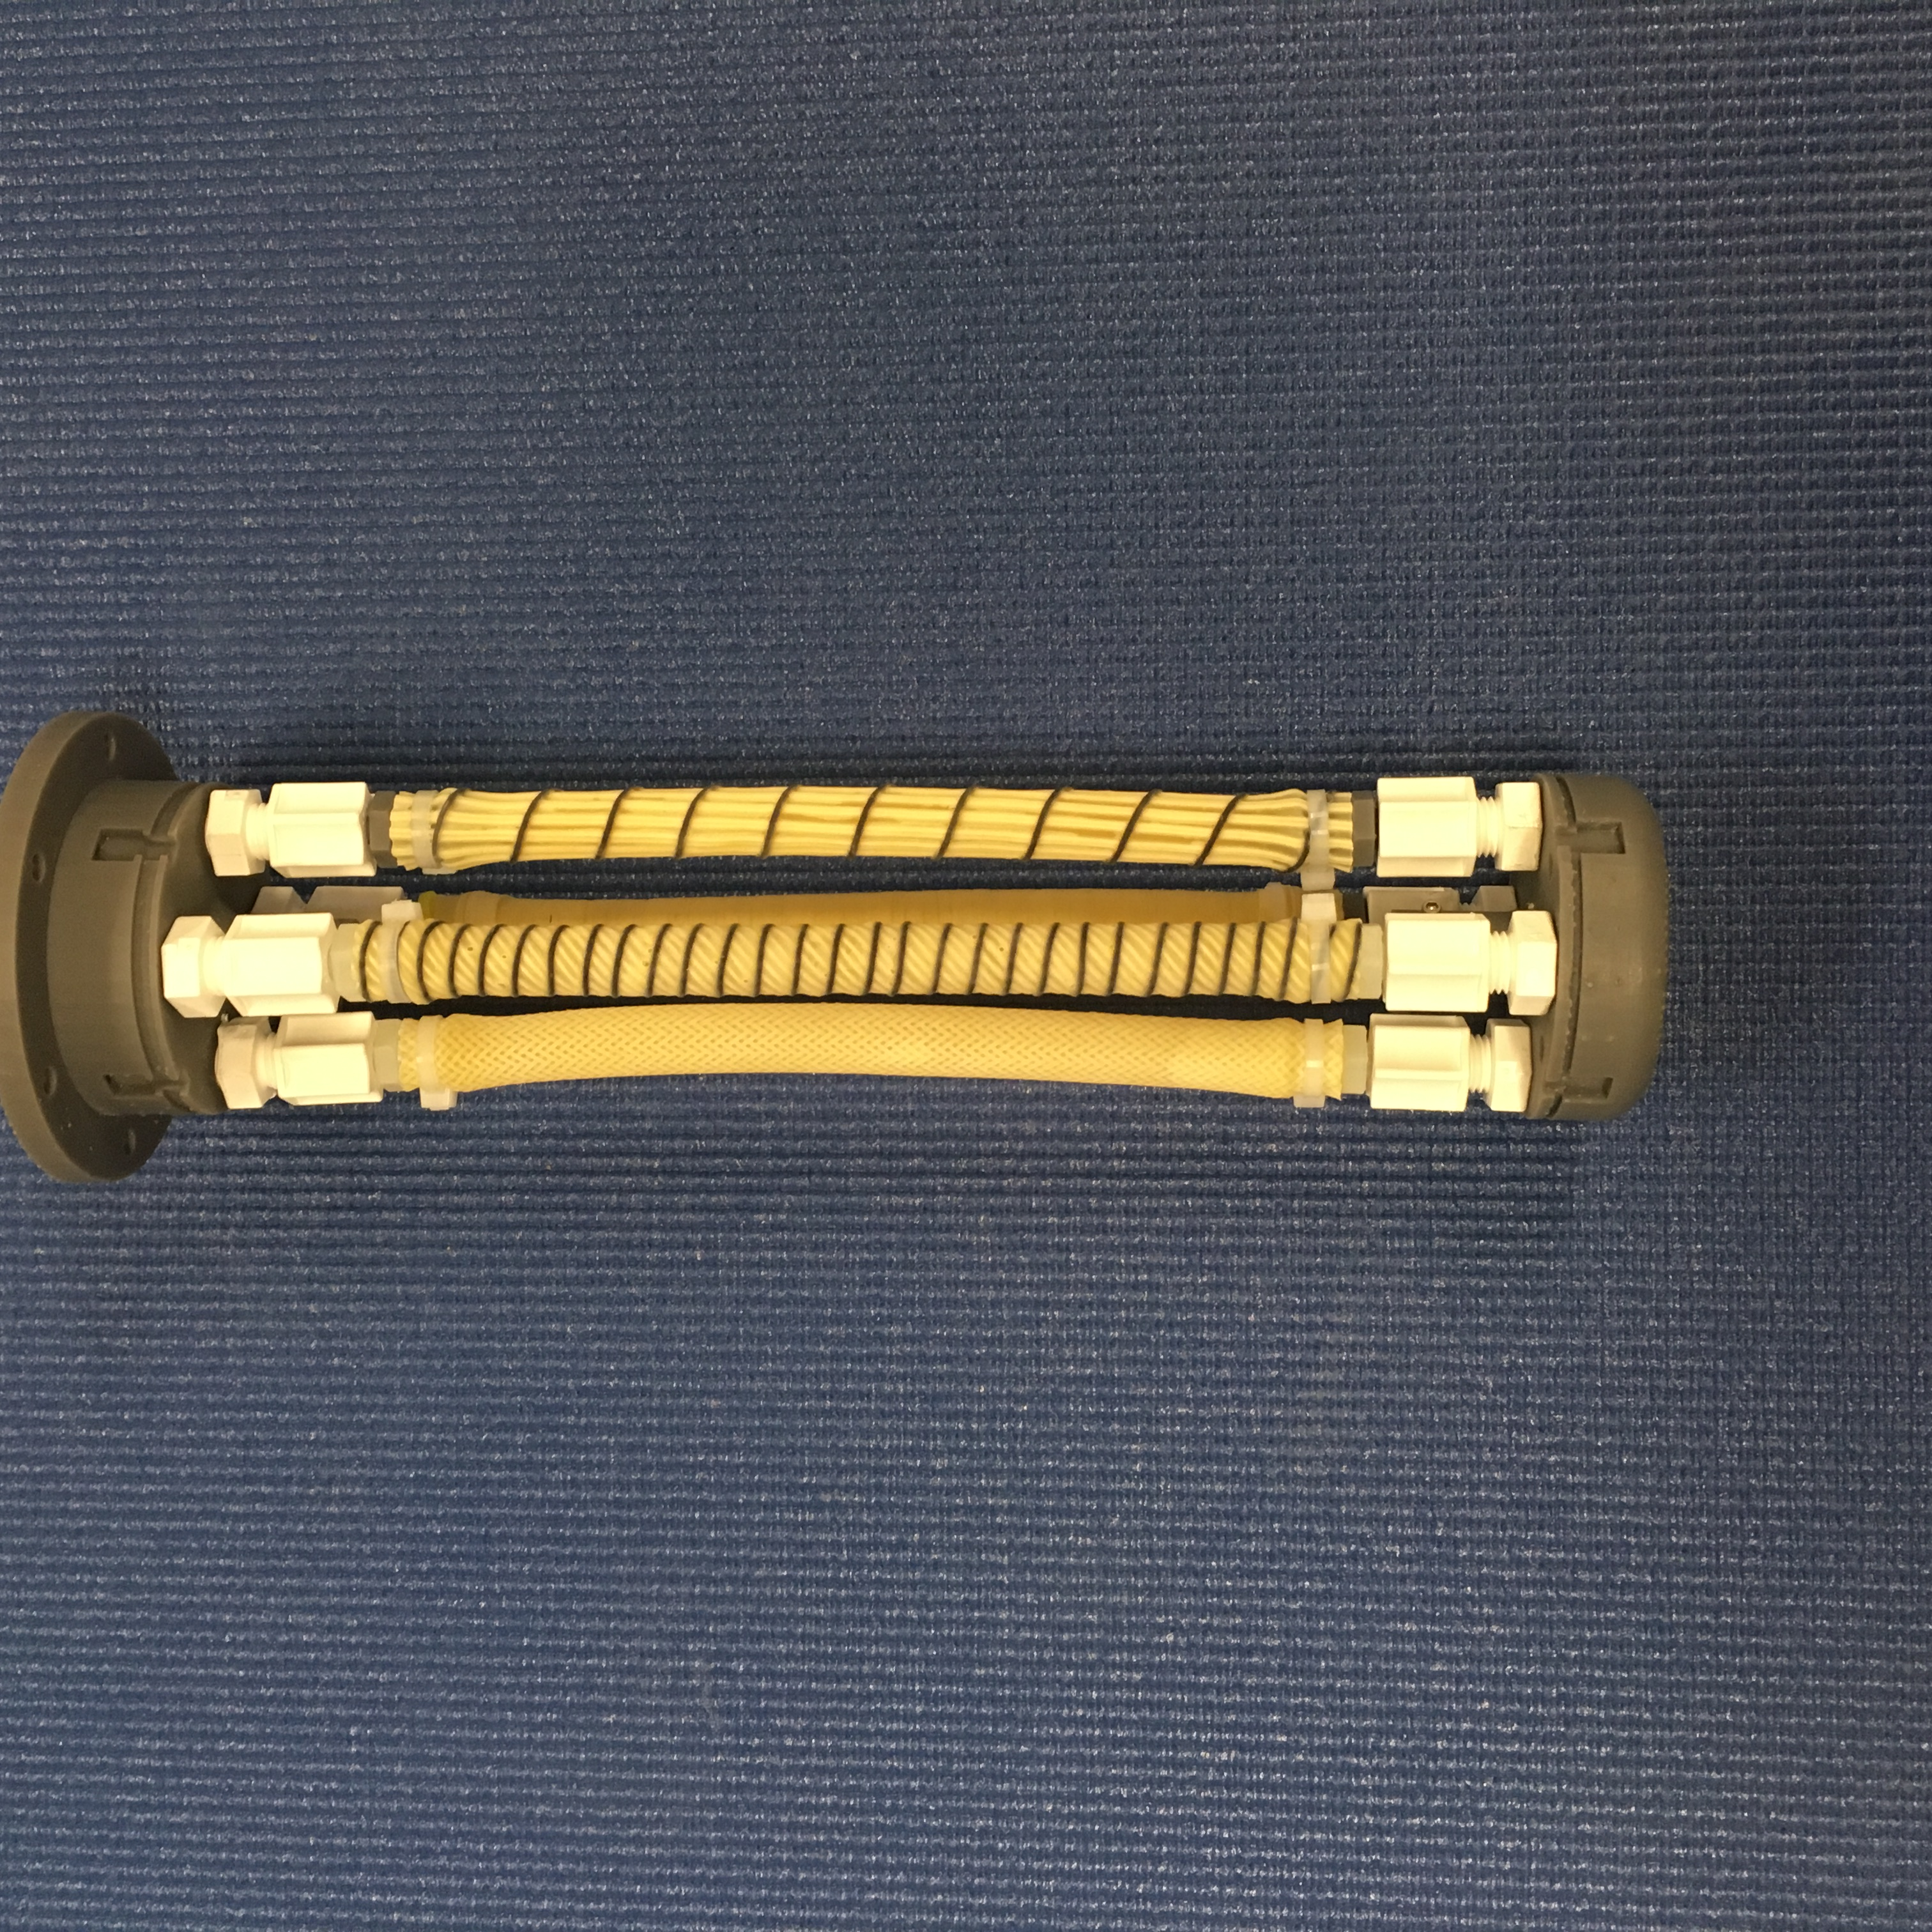
\includegraphics[width=\colWidth, angle=-90]{figures/free4.JPG}};
        \\
        };
    \end{tikzpicture}
    \caption{(a) A parallel system consisting of three FREE actuators attached to an end effector that is constrained to 2 DOF motion. A linear/rotary ball bearing allows the end effector to translate and rotate about a central shaft, while restricting motion in all other directions. (b) A parallel system consisting of four FREE actuators attached to an end effector that is constrained to 3 DOF motion. A centrally mounted spring-steel shaft  constrains the end effector to move on a 2D sub-manifold of 3D space, while also admitting rotations about its central axis. \Dan{these pictures/captions are placeholders. Will be replaced with much nicer versions with labels drawn on to show DOFs.}}
    \label{fig:modules}
\end{figure}

%% Equipment used in experiments
We conduct experiments on two parallel soft actuator systems. The first consists of three actuators constrained to 2 DOF motion (Figure \ref{fig:modules}a). The second consists of four actuators constrained 3 DOF motion (Figure \ref{fig:modules}b). So far, all of our experiments have been conducted using the three actuator system. In future experiments, we will apply the same model-based control approach to the less constrained system shown in figure \ref{fig:modules}b. During the experiments, the pressures inside the actuators are varied using pneumatic pressure regulars (Enfield TR-010-g10-s), and the displacement of the end effector is measured using a motion capture system (Phase Space Impulse X2E).

\newpage
\section{Main Experimental Insights}    \label{sec:insights}
% Main Experimental Insights
\newpage


% references section
\bibliographystyle{spmpsci}
\bibliography{references}

\end{document}
